\chapter{Results}
\label{chap:results}

% Talk about the calculations we did: parameters as before described with variable \lambda_{ir}; mean phonons, projections, see appendix A, etc...

\section{Classification of the excitations}
\label{sec:classification}

As previously noted in section \ref{sec:hamiltonian-and-basis}, only for zero charge-lattice couplings the eigenstates of the many-body Hamiltonian (\ref{eq:full-hamiltonian}) can be described as a direct product of purely electronic (an eigenstate of $H_{el}$) and phononic (an eigenstate of $H_{ph}$) states. 
That is, when the coupling parameters are zero the phonon number opreators $b_Rb^\dagger_R$ and $b_{ir}b^\dagger_{ir}$ have integer values with zero dispersion.
Increasing the value of the coupling parameters produces eigenstates with different mean phonon values and some finite dispersion.
In this scenario, the eigenstates are not striclty \textit{phononic}, \textit{electronic} or a product of both. 
The transition from this purely electronic or phononic states to a mixture of both, as a function of the coupling parameter $\lambda_{ir}$ is smooth.
That is, a hamiltonian with a small $\lambda_{ir}$ value will have only slighty different eigenstates from the uncoupled hamiltonian.
This mixed eigenstates can be thought of as largely phononic or electronic in nature.
For large coupling values the eigenstates are very different and can not be easily related to they uncoupled counterparts.
In figure \ref{fig:electr-proj} we show the first electronic state, for different $\lambda_{ir}$ values, projected with the first electronic state in the uncoupled system.
From this projection we can see that for small coupling values the electronic eigenstate remains largely unchanged.
In the middle coupling regime the change is strongest and then approaches zero at larger couplings.
This means that for small enough coupling values, this state remains \textit{electronic} in nature.
The vertical line in \ref{fig:electr-proj} at $\lambda_{ir}=0.1263$ eV, as will be discussed in section \ref{sec:grd-phonon-proj}, represents the $\lambda_{ir}$ value that reproduces the experimentally observed cluster distortion.
At this coupling value the electronic eigenstate has a projection with its uncoupled counterpart of $\sim 0.75$ which indicates that, although it has been changed considerably by the charge-lattice coupling, remains mostly electronic in nature.
Similar phenomenology can be observed for the rest of the excitations in this model.
Even though the eigenstates, for finite charge-lattice couplings, are not strictly electronic or phononic we will continue to refer to them as such since that interpretation remains useful in the regime of interest to us.
%
\begin{figure}
  \centering
  % GNUPLOT: LaTeX picture with Postscript
\begingroup
  \makeatletter
  \providecommand\color[2][]{%
    \GenericError{(gnuplot) \space\space\space\@spaces}{%
      Package color not loaded in conjunction with
      terminal option `colourtext'%
    }{See the gnuplot documentation for explanation.%
    }{Either use 'blacktext' in gnuplot or load the package
      color.sty in LaTeX.}%
    \renewcommand\color[2][]{}%
  }%
  \providecommand\includegraphics[2][]{%
    \GenericError{(gnuplot) \space\space\space\@spaces}{%
      Package graphicx or graphics not loaded%
    }{See the gnuplot documentation for explanation.%
    }{The gnuplot epslatex terminal needs graphicx.sty or graphics.sty.}%
    \renewcommand\includegraphics[2][]{}%
  }%
  \providecommand\rotatebox[2]{#2}%
  \@ifundefined{ifGPcolor}{%
    \newif\ifGPcolor
    \GPcolortrue
  }{}%
  \@ifundefined{ifGPblacktext}{%
    \newif\ifGPblacktext
    \GPblacktextfalse
  }{}%
  % define a \g@addto@macro without @ in the name:
  \let\gplgaddtomacro\g@addto@macro
  % define empty templates for all commands taking text:
  \gdef\gplbacktext{}%
  \gdef\gplfronttext{}%
  \makeatother
  \ifGPblacktext
    % no textcolor at all
    \def\colorrgb#1{}%
    \def\colorgray#1{}%
  \else
    % gray or color?
    \ifGPcolor
      \def\colorrgb#1{\color[rgb]{#1}}%
      \def\colorgray#1{\color[gray]{#1}}%
      \expandafter\def\csname LTw\endcsname{\color{white}}%
      \expandafter\def\csname LTb\endcsname{\color{black}}%
      \expandafter\def\csname LTa\endcsname{\color{black}}%
      \expandafter\def\csname LT0\endcsname{\color[rgb]{1,0,0}}%
      \expandafter\def\csname LT1\endcsname{\color[rgb]{0,1,0}}%
      \expandafter\def\csname LT2\endcsname{\color[rgb]{0,0,1}}%
      \expandafter\def\csname LT3\endcsname{\color[rgb]{1,0,1}}%
      \expandafter\def\csname LT4\endcsname{\color[rgb]{0,1,1}}%
      \expandafter\def\csname LT5\endcsname{\color[rgb]{1,1,0}}%
      \expandafter\def\csname LT6\endcsname{\color[rgb]{0,0,0}}%
      \expandafter\def\csname LT7\endcsname{\color[rgb]{1,0.3,0}}%
      \expandafter\def\csname LT8\endcsname{\color[rgb]{0.5,0.5,0.5}}%
    \else
      % gray
      \def\colorrgb#1{\color{black}}%
      \def\colorgray#1{\color[gray]{#1}}%
      \expandafter\def\csname LTw\endcsname{\color{white}}%
      \expandafter\def\csname LTb\endcsname{\color{black}}%
      \expandafter\def\csname LTa\endcsname{\color{black}}%
      \expandafter\def\csname LT0\endcsname{\color{black}}%
      \expandafter\def\csname LT1\endcsname{\color{black}}%
      \expandafter\def\csname LT2\endcsname{\color{black}}%
      \expandafter\def\csname LT3\endcsname{\color{black}}%
      \expandafter\def\csname LT4\endcsname{\color{black}}%
      \expandafter\def\csname LT5\endcsname{\color{black}}%
      \expandafter\def\csname LT6\endcsname{\color{black}}%
      \expandafter\def\csname LT7\endcsname{\color{black}}%
      \expandafter\def\csname LT8\endcsname{\color{black}}%
    \fi
  \fi
  \setlength{\unitlength}{0.0500bp}%
  \begin{picture}(6802.00,3968.00)%
    \gplgaddtomacro\gplbacktext{%
      \colorrgb{0.31,0.31,0.31}%
      \put(1078,751){\makebox(0,0)[r]{\strut{}\scriptsize 0}}%
      \colorrgb{0.31,0.31,0.31}%
      \put(1078,1313){\makebox(0,0)[r]{\strut{}\scriptsize 0.2}}%
      \colorrgb{0.31,0.31,0.31}%
      \put(1078,1876){\makebox(0,0)[r]{\strut{}\scriptsize 0.4}}%
      \colorrgb{0.31,0.31,0.31}%
      \put(1078,2438){\makebox(0,0)[r]{\strut{}\scriptsize 0.6}}%
      \colorrgb{0.31,0.31,0.31}%
      \put(1078,3000){\makebox(0,0)[r]{\strut{}\scriptsize 0.8}}%
      \colorrgb{0.31,0.31,0.31}%
      \put(1078,3562){\makebox(0,0)[r]{\strut{}\scriptsize 1}}%
      \colorrgb{0.31,0.31,0.31}%
      \put(1257,484){\makebox(0,0){\strut{}\scriptsize 0}}%
      \colorrgb{0.31,0.31,0.31}%
      \put(1669,484){\makebox(0,0){\strut{}\scriptsize 0.02}}%
      \colorrgb{0.31,0.31,0.31}%
      \put(2081,484){\makebox(0,0){\strut{}\scriptsize 0.04}}%
      \colorrgb{0.31,0.31,0.31}%
      \put(2493,484){\makebox(0,0){\strut{}\scriptsize 0.06}}%
      \colorrgb{0.31,0.31,0.31}%
      \put(2904,484){\makebox(0,0){\strut{}\scriptsize 0.08}}%
      \colorrgb{0.31,0.31,0.31}%
      \put(3316,484){\makebox(0,0){\strut{}\scriptsize 0.1}}%
      \colorrgb{0.31,0.31,0.31}%
      \put(3728,484){\makebox(0,0){\strut{}\scriptsize 0.12}}%
      \colorrgb{0.31,0.31,0.31}%
      \put(4140,484){\makebox(0,0){\strut{}\scriptsize 0.14}}%
      \colorrgb{0.31,0.31,0.31}%
      \put(4552,484){\makebox(0,0){\strut{}\scriptsize 0.16}}%
      \colorrgb{0.31,0.31,0.31}%
      \put(4964,484){\makebox(0,0){\strut{}\scriptsize 0.18}}%
      \colorrgb{0.31,0.31,0.31}%
      \put(5375,484){\makebox(0,0){\strut{}\scriptsize 0.2}}%
      \colorrgb{0.31,0.31,0.31}%
      \put(5787,484){\makebox(0,0){\strut{}\scriptsize 0.22}}%
      \colorrgb{0.31,0.31,0.31}%
      \put(6199,484){\makebox(0,0){\strut{}\scriptsize 0.24}}%
      \csname LTb\endcsname%
      \put(176,2227){\rotatebox{-270}{\makebox(0,0){\strut{}$\left|\braket{\psi_{el} (\lambda_{ir}=0)}{\psi_{el} (\lambda_{ir})}\right|$}}}%
      \put(3831,154){\makebox(0,0){\strut{}$\lambda_{ir}$ (eV)}}%
      \put(3934,3467){\makebox(0,0)[l]{\strut{}\scriptsize$\lambda_{ir}=0.1263$}}%
    }%
    \gplgaddtomacro\gplfronttext{%
    }%
    \gplbacktext
    \put(0,0){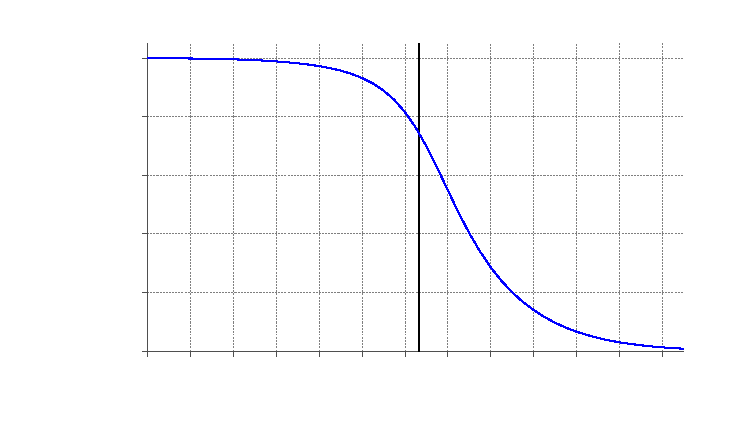
\includegraphics{images/electrProj}}%
    \gplfronttext
  \end{picture}%
\endgroup

  \caption[Projection of the first \textit{electronic} state with itself at $\lambda_{ir}=0$.]
  {Projection of the first \textit{electronic} state with itself at $\lambda_{ir}=0$.
    The vertical line denotes the experimentally relevant value $\lambda_{ir}=0.1263$ eV.}
  \label{fig:electr-proj}
\end{figure}

\section{Infrared spectra}

Figure \ref{fig:irSpectra} shows the infrared-active excitations for a range of $\lambda_{ir}$ values.
Note that, due to dipole selection rules, the excitation with two infrared phonons (green) is not visible with infared spectroscopy.

\begin{figure}
  \centering
  % GNUPLOT: LaTeX picture with Postscript
\begingroup
  \makeatletter
  \providecommand\color[2][]{%
    \GenericError{(gnuplot) \space\space\space\@spaces}{%
      Package color not loaded in conjunction with
      terminal option `colourtext'%
    }{See the gnuplot documentation for explanation.%
    }{Either use 'blacktext' in gnuplot or load the package
      color.sty in LaTeX.}%
    \renewcommand\color[2][]{}%
  }%
  \providecommand\includegraphics[2][]{%
    \GenericError{(gnuplot) \space\space\space\@spaces}{%
      Package graphicx or graphics not loaded%
    }{See the gnuplot documentation for explanation.%
    }{The gnuplot epslatex terminal needs graphicx.sty or graphics.sty.}%
    \renewcommand\includegraphics[2][]{}%
  }%
  \providecommand\rotatebox[2]{#2}%
  \@ifundefined{ifGPcolor}{%
    \newif\ifGPcolor
    \GPcolortrue
  }{}%
  \@ifundefined{ifGPblacktext}{%
    \newif\ifGPblacktext
    \GPblacktextfalse
  }{}%
  % define a \g@addto@macro without @ in the name:
  \let\gplgaddtomacro\g@addto@macro
  % define empty templates for all commands taking text:
  \gdef\gplbacktext{}%
  \gdef\gplfronttext{}%
  \makeatother
  \ifGPblacktext
    % no textcolor at all
    \def\colorrgb#1{}%
    \def\colorgray#1{}%
  \else
    % gray or color?
    \ifGPcolor
      \def\colorrgb#1{\color[rgb]{#1}}%
      \def\colorgray#1{\color[gray]{#1}}%
      \expandafter\def\csname LTw\endcsname{\color{white}}%
      \expandafter\def\csname LTb\endcsname{\color{black}}%
      \expandafter\def\csname LTa\endcsname{\color{black}}%
      \expandafter\def\csname LT0\endcsname{\color[rgb]{1,0,0}}%
      \expandafter\def\csname LT1\endcsname{\color[rgb]{0,1,0}}%
      \expandafter\def\csname LT2\endcsname{\color[rgb]{0,0,1}}%
      \expandafter\def\csname LT3\endcsname{\color[rgb]{1,0,1}}%
      \expandafter\def\csname LT4\endcsname{\color[rgb]{0,1,1}}%
      \expandafter\def\csname LT5\endcsname{\color[rgb]{1,1,0}}%
      \expandafter\def\csname LT6\endcsname{\color[rgb]{0,0,0}}%
      \expandafter\def\csname LT7\endcsname{\color[rgb]{1,0.3,0}}%
      \expandafter\def\csname LT8\endcsname{\color[rgb]{0.5,0.5,0.5}}%
    \else
      % gray
      \def\colorrgb#1{\color{black}}%
      \def\colorgray#1{\color[gray]{#1}}%
      \expandafter\def\csname LTw\endcsname{\color{white}}%
      \expandafter\def\csname LTb\endcsname{\color{black}}%
      \expandafter\def\csname LTa\endcsname{\color{black}}%
      \expandafter\def\csname LT0\endcsname{\color{black}}%
      \expandafter\def\csname LT1\endcsname{\color{black}}%
      \expandafter\def\csname LT2\endcsname{\color{black}}%
      \expandafter\def\csname LT3\endcsname{\color{black}}%
      \expandafter\def\csname LT4\endcsname{\color{black}}%
      \expandafter\def\csname LT5\endcsname{\color{black}}%
      \expandafter\def\csname LT6\endcsname{\color{black}}%
      \expandafter\def\csname LT7\endcsname{\color{black}}%
      \expandafter\def\csname LT8\endcsname{\color{black}}%
    \fi
  \fi
  \setlength{\unitlength}{0.0500bp}%
  \begin{picture}(6802.00,4534.00)%
    \gplgaddtomacro\gplbacktext{%
      \colorrgb{0.31,0.31,0.31}%
      \put(990,751){\makebox(0,0)[r]{\strut{}\scriptsize 0}}%
      \colorrgb{0.31,0.31,0.31}%
      \put(990,1191){\makebox(0,0)[r]{\strut{}\scriptsize 250}}%
      \colorrgb{0.31,0.31,0.31}%
      \put(990,1631){\makebox(0,0)[r]{\strut{}\scriptsize 500}}%
      \colorrgb{0.31,0.31,0.31}%
      \put(990,2070){\makebox(0,0)[r]{\strut{}\scriptsize 750}}%
      \colorrgb{0.31,0.31,0.31}%
      \put(990,2510){\makebox(0,0)[r]{\strut{}\scriptsize 1000}}%
      \colorrgb{0.31,0.31,0.31}%
      \put(990,2950){\makebox(0,0)[r]{\strut{}\scriptsize 1250}}%
      \colorrgb{0.31,0.31,0.31}%
      \put(990,3390){\makebox(0,0)[r]{\strut{}\scriptsize 1500}}%
      \colorrgb{0.31,0.31,0.31}%
      \put(990,3829){\makebox(0,0)[r]{\strut{}\scriptsize 1750}}%
      \colorrgb{0.31,0.31,0.31}%
      \put(990,4269){\makebox(0,0)[r]{\strut{}\scriptsize 2000}}%
      \colorrgb{0.31,0.31,0.31}%
      \put(1169,484){\makebox(0,0){\strut{}\scriptsize 0}}%
      \colorrgb{0.31,0.31,0.31}%
      \put(1588,484){\makebox(0,0){\strut{}\scriptsize 0.02}}%
      \colorrgb{0.31,0.31,0.31}%
      \put(2007,484){\makebox(0,0){\strut{}\scriptsize 0.04}}%
      \colorrgb{0.31,0.31,0.31}%
      \put(2426,484){\makebox(0,0){\strut{}\scriptsize 0.06}}%
      \colorrgb{0.31,0.31,0.31}%
      \put(2845,484){\makebox(0,0){\strut{}\scriptsize 0.08}}%
      \colorrgb{0.31,0.31,0.31}%
      \put(3263,484){\makebox(0,0){\strut{}\scriptsize 0.1}}%
      \colorrgb{0.31,0.31,0.31}%
      \put(3682,484){\makebox(0,0){\strut{}\scriptsize 0.12}}%
      \colorrgb{0.31,0.31,0.31}%
      \put(4101,484){\makebox(0,0){\strut{}\scriptsize 0.14}}%
      \colorrgb{0.31,0.31,0.31}%
      \put(4520,484){\makebox(0,0){\strut{}\scriptsize 0.16}}%
      \colorrgb{0.31,0.31,0.31}%
      \put(4939,484){\makebox(0,0){\strut{}\scriptsize 0.18}}%
      \colorrgb{0.31,0.31,0.31}%
      \put(5358,484){\makebox(0,0){\strut{}\scriptsize 0.2}}%
      \colorrgb{0.31,0.31,0.31}%
      \put(5777,484){\makebox(0,0){\strut{}\scriptsize 0.22}}%
      \colorrgb{0.31,0.31,0.31}%
      \put(6196,484){\makebox(0,0){\strut{}\scriptsize 0.24}}%
      \csname LTb\endcsname%
      \put(352,2510){\rotatebox{-270}{\makebox(0,0){\strut{}$\omega_i$ (cm$^{-1}$)}}}%
      \put(3787,154){\makebox(0,0){\strut{}$\lambda_{ir}$ (eV)}}%
      \put(3892,3988){\makebox(0,0)[l]{\strut{}\scriptsize$\lambda_{ir}=0.1263$}}%
    }%
    \gplgaddtomacro\gplfronttext{%
    }%
    \gplbacktext
    \put(0,0){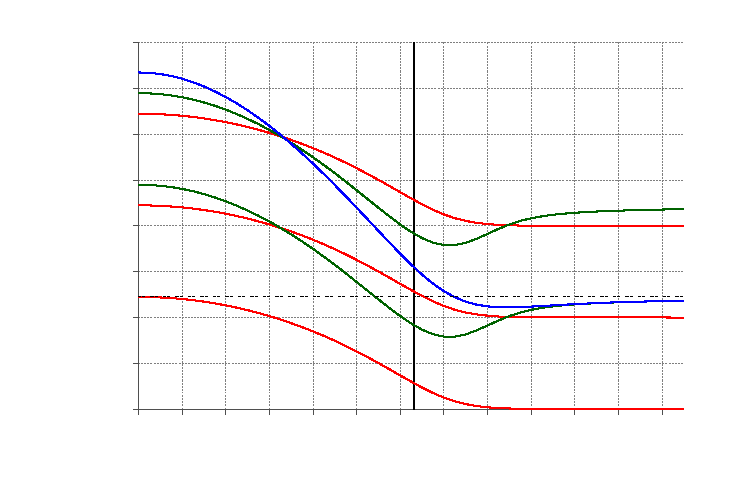
\includegraphics{images/irSpectra}}%
    \gplfronttext
  \end{picture}%
\endgroup

  \caption[Infrared-active excitations as a function of electron-lattice coupling.]
  {Infrared-active excitations as a function of electron-lattice coupling.
  The red, green and blue lines denote excitations which, initially, have one, two and three infrared phonons respectively.
  The horizontal dashed line is placed at the first infared-active excitation $\omega_i=612.4$ cm$^{-1}$ as a guide to the eye.}
  \label{fig:irSpectra}
\end{figure}


At large $\lambda_{ir}$ we recover the harmonic behaviour. This is analog to have a spring with a displaced equilibrium position.

\section{Projection into phonon coordinates}

\begin{figure}
  \centering
  % GNUPLOT: LaTeX picture with Postscript
\begingroup
  \makeatletter
  \providecommand\color[2][]{%
    \GenericError{(gnuplot) \space\space\space\@spaces}{%
      Package color not loaded in conjunction with
      terminal option `colourtext'%
    }{See the gnuplot documentation for explanation.%
    }{Either use 'blacktext' in gnuplot or load the package
      color.sty in LaTeX.}%
    \renewcommand\color[2][]{}%
  }%
  \providecommand\includegraphics[2][]{%
    \GenericError{(gnuplot) \space\space\space\@spaces}{%
      Package graphicx or graphics not loaded%
    }{See the gnuplot documentation for explanation.%
    }{The gnuplot epslatex terminal needs graphicx.sty or graphics.sty.}%
    \renewcommand\includegraphics[2][]{}%
  }%
  \providecommand\rotatebox[2]{#2}%
  \@ifundefined{ifGPcolor}{%
    \newif\ifGPcolor
    \GPcolortrue
  }{}%
  \@ifundefined{ifGPblacktext}{%
    \newif\ifGPblacktext
    \GPblacktextfalse
  }{}%
  % define a \g@addto@macro without @ in the name:
  \let\gplgaddtomacro\g@addto@macro
  % define empty templates for all commands taking text:
  \gdef\gplbacktext{}%
  \gdef\gplfronttext{}%
  \makeatother
  \ifGPblacktext
    % no textcolor at all
    \def\colorrgb#1{}%
    \def\colorgray#1{}%
  \else
    % gray or color?
    \ifGPcolor
      \def\colorrgb#1{\color[rgb]{#1}}%
      \def\colorgray#1{\color[gray]{#1}}%
      \expandafter\def\csname LTw\endcsname{\color{white}}%
      \expandafter\def\csname LTb\endcsname{\color{black}}%
      \expandafter\def\csname LTa\endcsname{\color{black}}%
      \expandafter\def\csname LT0\endcsname{\color[rgb]{1,0,0}}%
      \expandafter\def\csname LT1\endcsname{\color[rgb]{0,1,0}}%
      \expandafter\def\csname LT2\endcsname{\color[rgb]{0,0,1}}%
      \expandafter\def\csname LT3\endcsname{\color[rgb]{1,0,1}}%
      \expandafter\def\csname LT4\endcsname{\color[rgb]{0,1,1}}%
      \expandafter\def\csname LT5\endcsname{\color[rgb]{1,1,0}}%
      \expandafter\def\csname LT6\endcsname{\color[rgb]{0,0,0}}%
      \expandafter\def\csname LT7\endcsname{\color[rgb]{1,0.3,0}}%
      \expandafter\def\csname LT8\endcsname{\color[rgb]{0.5,0.5,0.5}}%
    \else
      % gray
      \def\colorrgb#1{\color{black}}%
      \def\colorgray#1{\color[gray]{#1}}%
      \expandafter\def\csname LTw\endcsname{\color{white}}%
      \expandafter\def\csname LTb\endcsname{\color{black}}%
      \expandafter\def\csname LTa\endcsname{\color{black}}%
      \expandafter\def\csname LT0\endcsname{\color{black}}%
      \expandafter\def\csname LT1\endcsname{\color{black}}%
      \expandafter\def\csname LT2\endcsname{\color{black}}%
      \expandafter\def\csname LT3\endcsname{\color{black}}%
      \expandafter\def\csname LT4\endcsname{\color{black}}%
      \expandafter\def\csname LT5\endcsname{\color{black}}%
      \expandafter\def\csname LT6\endcsname{\color{black}}%
      \expandafter\def\csname LT7\endcsname{\color{black}}%
      \expandafter\def\csname LT8\endcsname{\color{black}}%
    \fi
  \fi
  \setlength{\unitlength}{0.0500bp}%
  \begin{picture}(8502.00,2834.00)%
    \gplgaddtomacro\gplbacktext{%
      \csname LTb\endcsname%
      \put(1210,918){\makebox(0,0)[r]{\strut{}\scriptsize -0.3}}%
      \put(1210,1158){\makebox(0,0)[r]{\strut{}\scriptsize -0.2}}%
      \put(1210,1397){\makebox(0,0)[r]{\strut{}\scriptsize -0.1}}%
      \put(1210,1636){\makebox(0,0)[r]{\strut{}\scriptsize 0}}%
      \put(1210,1876){\makebox(0,0)[r]{\strut{}\scriptsize 0.1}}%
      \put(1210,2115){\makebox(0,0)[r]{\strut{}\scriptsize 0.2}}%
      \put(1210,2355){\makebox(0,0)[r]{\strut{}\scriptsize 0.3}}%
      \put(1397,484){\makebox(0,0){\strut{}\scriptsize -0.4}}%
      \put(1742,484){\makebox(0,0){\strut{}\scriptsize -0.2}}%
      \put(2088,484){\makebox(0,0){\strut{}\scriptsize 0}}%
      \put(2434,484){\makebox(0,0){\strut{}\scriptsize 0.2}}%
      \put(2779,484){\makebox(0,0){\strut{}\scriptsize 0.4}}%
      \put(176,1636){\rotatebox{-270}{\makebox(0,0){\strut{}$u_{R}$ (\AA)}}}%
      \put(2088,154){\makebox(0,0){\strut{}$u_{ir}$ (\AA)}}%
      \put(1105,2720){\makebox(0,0)[l]{\strut{}$\lambda_{ir} = 0.00$ eV}}%
    }%
    \gplgaddtomacro\gplfronttext{%
    }%
    \gplgaddtomacro\gplbacktext{%
      \csname LTb\endcsname%
      \put(3088,918){\makebox(0,0)[r]{\strut{}}}%
      \put(3088,1158){\makebox(0,0)[r]{\strut{}}}%
      \put(3088,1397){\makebox(0,0)[r]{\strut{}}}%
      \put(3088,1636){\makebox(0,0)[r]{\strut{}}}%
      \put(3088,1876){\makebox(0,0)[r]{\strut{}}}%
      \put(3088,2115){\makebox(0,0)[r]{\strut{}}}%
      \put(3088,2355){\makebox(0,0)[r]{\strut{}}}%
      \put(3288,484){\makebox(0,0){\strut{}\scriptsize -0.4}}%
      \put(3721,484){\makebox(0,0){\strut{}\scriptsize -0.2}}%
      \put(4154,484){\makebox(0,0){\strut{}\scriptsize 0}}%
      \put(4586,484){\makebox(0,0){\strut{}\scriptsize 0.2}}%
      \put(5019,484){\makebox(0,0){\strut{}\scriptsize 0.4}}%
      \put(3066,1636){\rotatebox{-270}{\makebox(0,0){\strut{}}}}%
      \put(4153,154){\makebox(0,0){\strut{}$u_{ir}$ (\AA)}}%
      \put(3400,2720){\makebox(0,0)[l]{\strut{}$\lambda_{ir} = 0.1263$ eV}}%
    }%
    \gplgaddtomacro\gplfronttext{%
    }%
    \gplgaddtomacro\gplbacktext{%
      \csname LTb\endcsname%
      \put(5681,918){\makebox(0,0)[r]{\strut{}}}%
      \put(5681,1158){\makebox(0,0)[r]{\strut{}}}%
      \put(5681,1397){\makebox(0,0)[r]{\strut{}}}%
      \put(5681,1636){\makebox(0,0)[r]{\strut{}}}%
      \put(5681,1876){\makebox(0,0)[r]{\strut{}}}%
      \put(5681,2115){\makebox(0,0)[r]{\strut{}}}%
      \put(5681,2355){\makebox(0,0)[r]{\strut{}}}%
      \put(5872,484){\makebox(0,0){\strut{}\scriptsize -0.4}}%
      \put(6246,484){\makebox(0,0){\strut{}\scriptsize -0.2}}%
      \put(6620,484){\makebox(0,0){\strut{}\scriptsize 0}}%
      \put(6994,484){\makebox(0,0){\strut{}\scriptsize 0.2}}%
      \put(7368,484){\makebox(0,0){\strut{}\scriptsize 0.4}}%
      \put(5659,1636){\rotatebox{-270}{\makebox(0,0){\strut{}}}}%
      \put(6620,154){\makebox(0,0){\strut{}$u_{ir}$ (\AA)}}%
      \put(5951,2720){\makebox(0,0)[l]{\strut{}$\lambda_{ir} = 0.25$ eV}}%
    }%
    \gplgaddtomacro\gplfronttext{%
      \csname LTb\endcsname%
      \put(7679,704){\makebox(0,0)[l]{\strut{} 0}}%
      \put(7679,1014){\makebox(0,0)[l]{\strut{} 0.02}}%
      \put(7679,1325){\makebox(0,0)[l]{\strut{} 0.04}}%
      \put(7679,1636){\makebox(0,0)[l]{\strut{} 0.06}}%
      \put(7679,1947){\makebox(0,0)[l]{\strut{} 0.08}}%
      \put(7679,2258){\makebox(0,0)[l]{\strut{} 0.1}}%
      \put(7679,2569){\makebox(0,0)[l]{\strut{} 0.12}}%
    }%
    \gplbacktext
    \put(0,0){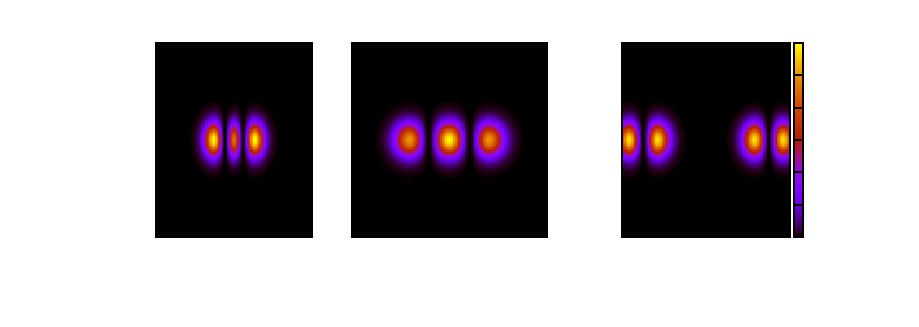
\includegraphics{images/phononProj2ir}}%
    \gplfronttext
  \end{picture}%
\endgroup

  \caption{Projection into phonon coordinates of the state with 2 infrared phonons.}
  \label{fig:ph-second_infrared}
\end{figure}

\begin{figure}[ht!]
  \centering
  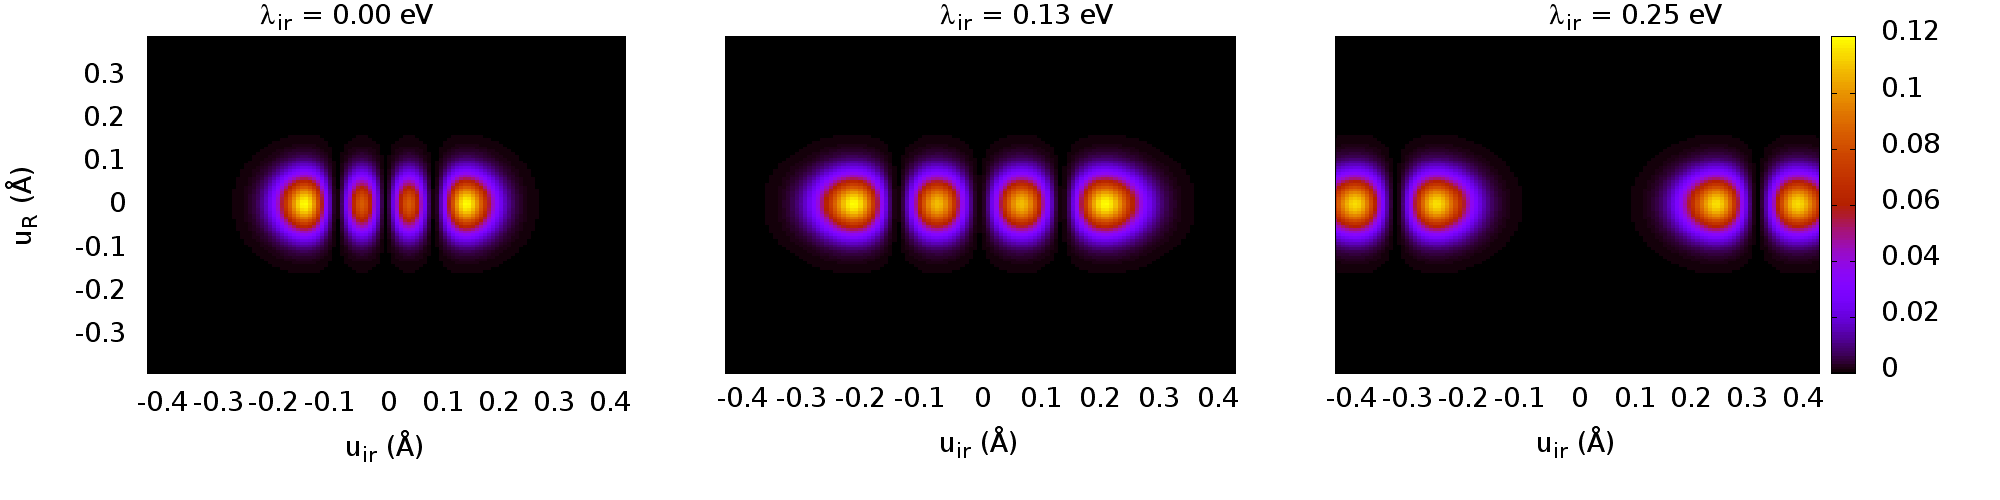
\includegraphics[width=0.8\textwidth]{images/ph-third_infrared.png}
  \caption{Projection into phonon coordinates of the state with 3 infrared phonons.}
  \label{fig:ph-third_infrared}
\end{figure}

\section{Isotopic shifts}

The isotopic shifts are different:

\begin{figure}[ht!]
  \centering
  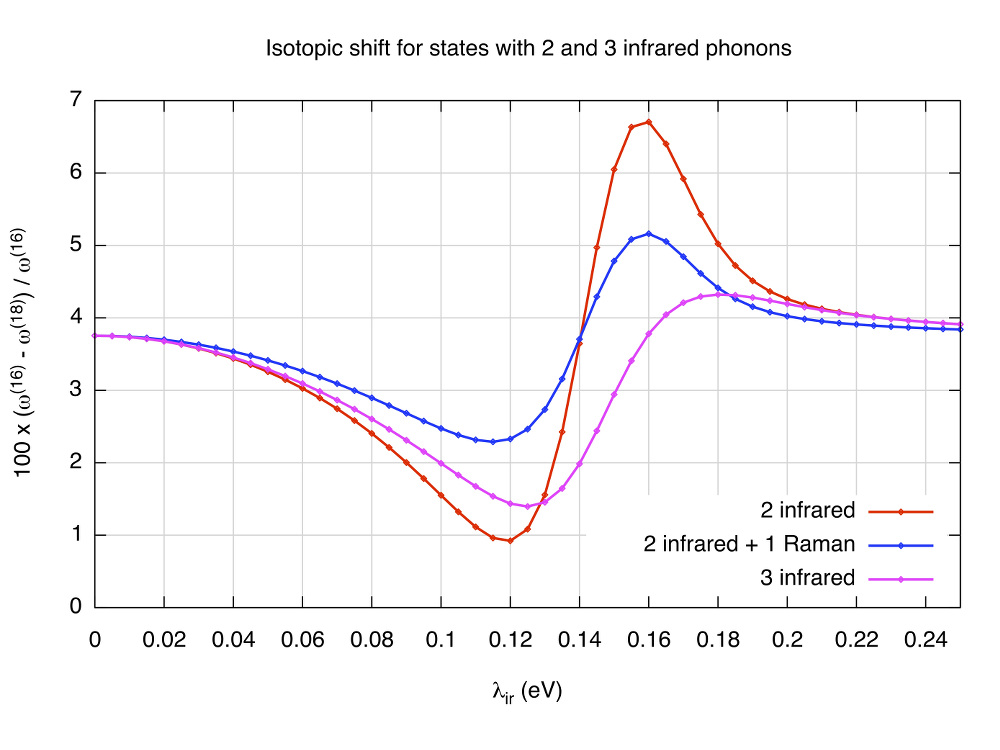
\includegraphics[width=0.8\textwidth]{images/isot-2_3ir.jpg}
  \caption{Isotopic shifts}
  \label{fig:isot-2_3ir}
\end{figure}
